\chapter{Preliminares}
\label{chapter:preliminares}

En este capítulo se presenta el marco teórico de este trabajo, dando un panorama
general de cada una de las disciplinas abordadas e introduciendo los conceptos
básicos y fundamentales para entender el proyecto. Se comienza con la definición
de la taxonomía del campo de estudio y luego se abordan los conceptos claves de
la tarea de clasificación multi-etiquetas y su aplicación en ambientes de flujos
continuos. Muchos de los algoritmos y métricas de evaluación son parte de la
configuración experimental, y por tanto, serán mencionados nuevamente en
capítulos posteriores.

\section{Taxonomía del Campo de Estudio}

\begin{figure}[htbp]
	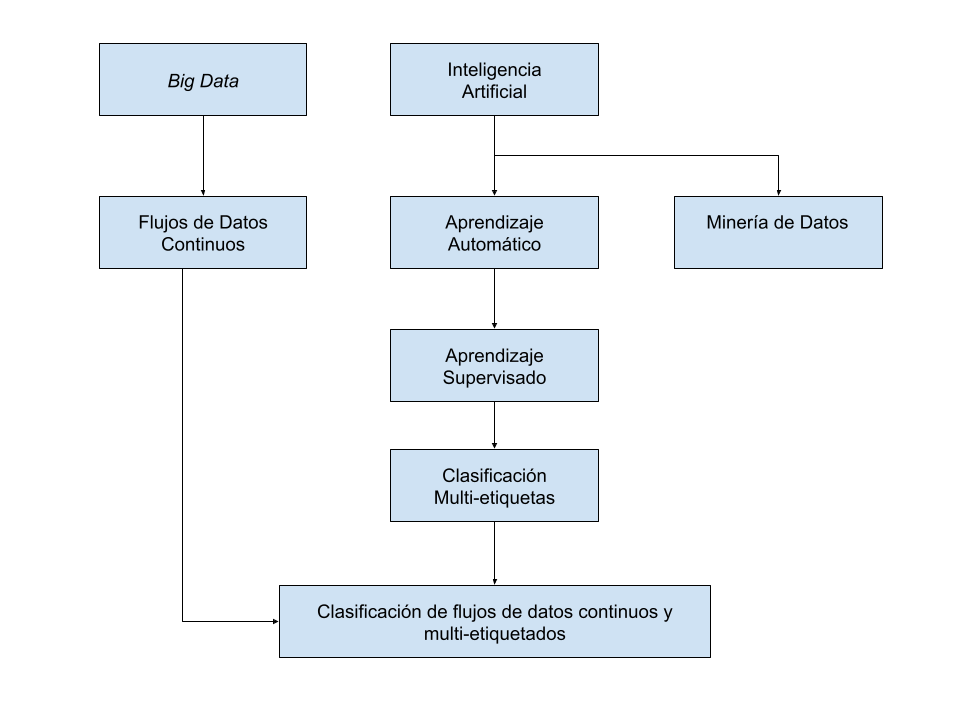
\includegraphics[width=.9\linewidth]{figures/study_field_taxonomy_v2.png}
	\centering
	\caption{Taxonomía del campo de estudio.}
	\label{fig:campo_estudio}
\end{figure}

En pocas palabras, el presente trabajo de investigación se enmarca en las áreas
de \textit{big data} y minería de datos, con aplicación en escenarios de
\textit{streaming} o flujos continuos de datos y abordando clasificaciones
multi-etiquetas.

La figura~\ref{fig:campo_estudio} es un esquema que ilustra la taxonomía del
campo de estudio y la interrelación entre las áreas de investigación
involucradas.

\section{Clasificación Multi-etiquetas}

A diferencia del aprendizaje automático tradicional (ver
anexo~\ref{anexo:clasificacion_tradicional}), que usa datos de etiqueta única
para representar objetos del mundo real, cada instancia en el aprendizaje
multi-etiquetas representa un único objeto, pero puede contener más de una
etiqueta. Por consiguiente, la tarea de clasificación consiste en hallar una
función que logre asignar a cada objeto, nuevo y desconocido, el conjunto de
etiquetas que lo caracteriza.

En este apartado se da una definición formal, se detallan las características de
un conjunto de datos multi-etiquetados y se  describen algunos métodos
tradicionales de clasificación multi-etiquetas junto con sus ventajas,
desventajas, aplicaciones y motivaciones.

\subsection{Definición}
\label{mll_def_formal}

Asumiendo que $X=\mathbb{R}^{d}$ denota el espacio de instancias $d$
dimensional, y que $Y = \{y_{1}, y_{2}, \dots, y_{q}\}$ denota el espacio de
etiquetas con $q$ etiquetas posibles, la tarea de clasificación multi-etiquetas
consiste en entrenar un conjunto $D = \{(x_{i}, Y_{i}) \mid 1 \leq i \leq m\}$
para hallar una función $h$ tal que $h: X \rightarrow 2^y$. A su vez, $X_{i}$ es
un vector de atributos $d$ dimensional definido como $(x_{i1}, x_{i2}, \dots,
	x_{id})$. $Y_{i}$, por su parte, es el conjunto de etiquetas asociadas a la
instancia $X_{i}$. Luego, para cada instancia desconocida $x \in X$ el
clasificador $h$ predice $h(x) \subseteq Y$ que representa el conjunto de
etiquetas hallado para $x$.

A su vez, se definen un conjunto de métricas que describen el grado de
multi-etiquetado que tiene un conjunto de datos dado, o en otras palabras, hasta
qué punto cada ejemplo posee más de una etiqueta. Algunas de ellas son:

\begin{description}
	\item{Cardinalidad de etiquetas}: Es el promedio de etiquetas por instancia
	      del conjunto de datos. Se define como:
	      \begin{equation}
		      \label{eq:mll_card}
		      CardE(D) = \frac{1}{m} \sum_{i=1}^{m} \left\|Y_{i}\right\|
	      \end{equation}
	      Por lo tanto, a mayor el valor de cardinalidad, mayor es el número de
	      etiquetas de una instancia. Por ejemplo, si $CardE = 1$, entonces la
	      mayoría de ejemplos tiene una única etiqueta y, por consiguiente, se puede
	      decir que la colección tiene un grado bajo de multi-etiquetado.
	\item{Densidad de etiquetas}: Es la cardinalidad de etiquetas normalizada al
	      número total de etiquetas de $D$ y se define como:
	      \begin{equation}
		      DenE(D) = \frac{CardE(D)}{\left\|Y\right\|}
	      \end{equation}
	      Así pues, un valor alto de densidad significaría que cada instancia puede
	      ser una buena representación de las etiquetas del conjunto. De la misma
	      manera, un valor bajo suele implicar dispersión, esto es, que la mayoría
	      de las instancias tienen un subconjunto acotado de las etiquetas.
	\item{Diversidad de etiquetas}: Es el número de conjuntos de etiquetas
	      unívocos que aparecen en instancias de $D$. Se define como:
	      \begin{equation}
		      DivE(D) = \left\|\{Y \mid \exists x: (x, Y) \in D\}\right\|
	      \end{equation}
	      Aquí la interpretación es que, a mayor el valor de diversidad, menor es la
	      constancia con la que las etiquetas aparecen en las instancias. De manera
	      similar a la cardinalidad, el valor de diversidad también puede
	      normalizarse por el número de instancias del conjunto de datos:
	      \begin{equation}
		      DivEProm(D) = \frac{DivE(D)}{\left\|D\right\|}
	      \end{equation}
\end{description}

\subsection{Algoritmos}

Como se había anticipado en la sección~\ref{intro_mll}, la tarea de aprendizaje
sobre datos multi-etiquetados puede ser encarada siguiendo dos grandes enfoques,
llamados \comillas{Transformación del Problema} y \comillas{Adaptación del
	Algoritmo}. A continuación se describen ambos enfoques y algunos de sus
algoritmos más representativos.

\subsubsection{Transformación del Problema}

Esta categoría engloba al conjunto de algoritmos que abordan el problema de
clasificación multi-etiquetas transformándolo en múltiples problemas de
clasificación de única etiqueta, lo cual permite aplicar algoritmos de
clasificación convencionales. Tres de estos métodos son particularmente
relevantes para este trabajo: \comillas{\acrfull{br}}, \comillas{\acrfull{cc}} y
\comillas{\acrfull{lp}}.

\paragraph{\acrfull{br}}

El algoritmo de Relevancia Binaria, conocido como \textit{\acrlong{br}} en la
literatura, es un enfoque que consiste en descomponer la tarea de clasificación
\acrshort{mll} en $\left\|q\right\|$ clasificadores binarios, independientes y
de etiqueta única.  A partir de esta transformación se puede seleccionar
cualquier algoritmo de clasificación tradicional como clasificador base del
problema (ver los algoritmos presentados en~\ref{clasificacion_algoritmos}).
Cada clasificador binario $g_{j}$ es entrenado con todas las instancias de la
colección, pero incluyendo solo la etiqueta $j$, la cual se activa o desactiva
de acuerdo a si es relevante a la instancia. Luego la predicción de una
instancia desconocida se realiza combinando las salidas de cada clasificador
individual, esto es:

\begin{equation}
	Y = {y_{j} \mid g_{j}(x) > 0, 1 \leq j \leq q}
\end{equation}

Llegado el caso en que ninguno de los clasificadores retornen etiquetas activas,
el conjunto $Y$ será vacío.

Este enfoque se dice que es de primer orden (ver sección~\ref{estrategias_mll})
y no tiene en cuenta las correlaciones o interdependencias entre etiquetas. Este
es uno de los principales inconvenientes de este algoritmo porque, en este tipo
de problemas de \acrshort{mll}, es usual hallar que determinadas etiquetas se
activan en conjunto con mayor probabilidad. Pese a ello, \acrshort{br} es un
enfoque muy utilizado \cite{zhang_review_2014} ya que es simple de implementar,
intuitivo y computacionalmente poco costoso en comparación con algoritmos que sí
tienen en cuenta la relación entre etiquetas.

\paragraph{\acrfull{cc}}

Las cadenas de clasificadores o \textit{\acrlong{cc}}
\cite{read_classifier_2011} es una técnica que convierte el problema de
\acrshort{mll} en una \comillas{cadena} de problemas de clasificación binaria,
tal que el siguiente clasificador de la cadena posee las predicciones de los
anteriores. En principio, la división del conjunto de datos es similar a la que
se hace en el enfoque anterior, designando un clasificador por cada etiqueta.
Durante el entrenamiento, el clasificador inicial, seleccionado aleatoriamente,
usa de entrada los atributos originales, tal como el clasificador \acrshort{br}.
Luego la salida de este clasificador es añadida al espacio de atributos como un
atributo más de cada instancia, para que posteriormente, estos atributos sean la
entrada del siguiente clasificador, el cual también es seleccionado al azar.
Este proceso es repetido hasta completar todos los clasificadores.  Como se
puede observar, lo que se produce es un \comillas{encadenamiento} de
clasificadores, el cual no es accidental y tiene como fin conservar la
dependencia entre etiquetas: en el entrenamiento se van acumulando las salidas
de los clasificadores anteriores de tal manera que el siguiente clasificador
absorbe la correlación entre las etiquetas de los anteriores.

Cabe notar que en esta técnica cobra especial importancia el ordenamiento de los
clasificadores, ya que este orden tiene un impacto directo sobre el resultado de
la predicción. En otras palabras, si el ordenamiento se modifica, el modelo
final otorgará resultados diferentes. Para salvar esta dificultad se han
propuesto modelos como \acrfull{ecc}. El mismo genera un conjunto de modelos de
\acrshort{cc} con distintos ordenamientos y entrenados con diversos subconjuntos
de datos, generados con reemplazo o no. Durante la predicción, cada cadena
produce un conjunto de etiquetas, que son los votos, y la salida final será
computada por un algoritmo que combine cada salida individual.

\paragraph{\acrfull{lp}}

El conjunto de potencias de etiquetas o \textit{\acrlong{lp}}
\cite{tsoumakas_random_2011} es una técnica que se encarga de transformar el
problema de \acrshort{mll} en uno de clasificación multi-clase y así poder
abordarlo con algoritmos de este tipo. La clasificación multi-clase es un
enfoque usado para tratar con ejemplos en donde la etiqueta es única, pero
cuenta con más de dos clases. Un ejemplo de este tipo de problemas es el de
análisis de sentimiento de texto, en donde las clases pueden ser
\comillas{positivo}, \comillas{negativo} y \comillas{neutral}. En \acrshort{lp}
cada etiqueta indica el subconjunto de etiquetas de la instancia. Esto es
beneficioso en cuanto a que se logra preservar la dependencia entre etiquetas.
Sin embargo, el modelo tiene algunas dificultades.  En primer lugar, el espacio
de clases posibles es exponencial y su cantidad de clases puede llegar a ser de
$2^{\left\|q\right\|}$ como máximo. A su vez, pueden llegar a arribar ejemplos
con una combinación de etiquetas que el modelo no recibió durante el
entrenamiento, por lo cual no logra generalizar lo suficiente y se lo considera
un modelo incompleto. A fin de sobrepasar estas complicaciones se desarrolló la
técnica de \comillas{Conjuntos Podados} o \comillas{\acrfull{ps}}. La misma
consiste en preservar para la clasificación aquellos subconjuntos de etiquetas
que son más frecuentes en la colección, y eliminar los demás. Con esto se logra
disminuir considerablemente el espacio de clases y disminuye la complejidad
computacional, tanto durante el entrenamiento como durante la predicción.

\subsubsection{Adaptación del Algoritmo}

Además del enfoque de transformación del problema, algunos autores abordan la
clasificación multi-etiquetas a partir de la adaptación de algoritmos clásicos y
bien conocidos a este tipo de escenarios. La categoría engloba al conjunto de
algoritmos que acometen el problema de \acrshort{mll} mediante la modificación
de algoritmos de etiqueta única para que sean capaces de manejar la nueva
naturaleza de los datos en estas tareas. Las modificaciones que se introducen
pueden variar en complejidad según el algoritmo tratado y las características de
la colección.  Se han adaptado una diversa cantidad de algoritmos incluyendo
aquellos basados en redes neuronales, árboles, métodos probabilísticos, entre
otros \cite{herrera_multilabel_2016}.  Por mencionar algunos ejemplos,
\citeauthor{gargiulo_deep_2018} usan redes neuronales profundas para clasificar
documentos de texto libre y comparan su funcionamiento variando el número de
etiquetas y aprovechando su estructura jerárquica \cite{gargiulo_deep_2018}.
Asimismo, \citeauthor{tanaka_multi-label_2015} agregan al algoritmo de
\acrshort{br} la capacidad de capturar relaciones entre etiquetas a través del
uso de árboles de decisión y lo aplican en el área de la genómica
\cite{tanaka_multi-label_2015}.

En lo que confiere a ambientes de flujos continuos de datos una de las técnicas
más populares en la literatura es la de Árbol de Hoeffding o
\textit{\acrfull{ht}} \cite{domingos_mining_2002}, que a diferencia de los
algoritmos convencionales de árboles de decisión, aborda los datos de manera
incremental. Así pues, en lugar de realizar decisiones de corte de acuerdo a los
datos previamente almacenados, el algoritmo de \acrshort{ht} espera a tener una
cantidad suficiente de instancias para realizar el corte, con un cierto grado de
confianza. Esto significa que ya no es necesario guardar todos los datos de la
colección y que mantener una serie de estadísticas es suficiente para realizar
la clasificación. Otra de las propiedades a destacar de este método es que, en
la teoría, se puede entrenar un árbol cuyo rendimiento se aproxime al generado
en un ambiente de \textit{batch}, con la suficiente cantidad de datos
\cite{bifet_machine_2018}.

A partir de esto, y buscando sacar provecho de las ventajas mencionadas,
\citeauthor{read_scalable_2012} decidieron adaptar este algoritmo a problemas de
multi-etiquetas y desarrollaron el algoritmo llamado Árbol de Hoeffding
Multi-etiquetado o \textit{\acrfull{mlht}} \cite{read_scalable_2012}. Esto lo
consiguen a partir de rediseñar la fórmula de ganancia de información (ver
fórmula~\ref{eq:gan_c45}) de tal manera de reflejar en el cálculo de la entropía
el impacto de todas las clases a las cuales el ejemplo no pertenece. Desde que
fue introducido en el año \citeyear{read_scalable_2012}, \acrshort{mlht} ha sido
usado como modelo de comparación en reiteradas oportunidades
\cite{sousa_multi-label_2018} y es uno de los métodos más populares para atacar
problemas de \acrshort{mll} en ambientes de flujo continuo de datos.

Otro algoritmo muy popular para abordar este tipo de problemas y que también se
basa en árboles de decisión incrementales es el llamado \acrshort{isoup} (siglas
del inglés \textit{\acrlong{isoup}}) \cite{osojnik_multi-label_2017}. El mismo
fue desarrollado inicialmente para hacer regresión de múltiples objetivos y
luego fue adaptado a tareas de \acrshort{mll}. Una de las novedades que
introduce es el uso de un perceptrón adaptativo en las hojas del árbol, lo cual
le da la versatilidad de poder trabajar tanto con problemas de clasificación
como de regresión.

\todo[inline]{Explicación de enfoques de ensambles? (ebr, ecc, elp)}

\subsection{Evaluación}
\label{mll_evaluacion}

Como se describe en el anexo~\ref{evaluacion_metricas}, en escenarios de
clasificación tradicionales el poder de generalización de un modelo es evaluado
a partir de métricas tales como la exactitud o la exhaustividad las cuales
trabajan con una única etiqueta. Una predicción multi-etiquetada, por el
contrario, carga con la complejidad de que cada ejemplo puede ser asociado a más
de una o dos etiquetas. Esto implica que ya no se puede trabajar con la
presunción de que una clasificación solo puede ser correcta o incorrecta. De lo
contrario, se incursionaría en una evaluación excesivamente rigurosa. Por este
motivo, en el campo de \acrshort{mll} se han diseñado una serie de métricas
nuevas y específicas para abordar este tipo de problemas, y se clasifican en dos
grupos: existen las métricas \comillas{basadas en ejemplos}, que son computadas
por cada instancia y luego promediadas; y las métricas \comillas{basadas en
	etiquetas}, las cuales son calculadas para cada etiqueta por separado y
devuelven el promedio micro o el promedio macro.

A continuación se describe en detalle ambas categorías, incluyendo métricas
presentadas por cada enfoque, junto con su definición formal y una
interpretación de la evaluación que proveen.

\subsubsection{Métricas basadas en Ejemplos}

En esta categoría se hallan las métricas que evalúan la calidad de la
clasificación ejemplo por ejemplo y determinan qué tan buena es la clasificación
sobre los distintos ejemplos. Tienen en común que comparan las etiquetas de la
predicción contra las etiquetas reales para cada instancia y luego combinan la
salida aplicando la media sobre el total de instancias. Entre ellas se
encuentran las siguientes:

\paragraph{\textit{Hamming Loss}}

Esta es una de las métricas más populares en la literatura y se encarga de
evaluar la proporción de pares instancia-etiqueta incorrectamente clasificados,
es decir, toma en cuenta para el conteo tanto si se marcó como irrelevante una
etiqueta relevante o si, por el contrario, se activó una etiqueta que no era
relevante. Se define como:

\begin{equation}
	HLoss = \frac{1}{m} \sum_{i=1}^{m} \left\|h(x_{i}) \triangle Y_{i}\right\|
\end{equation}

Aquí el símbolo \comillas{$\triangle$} es la diferencia simétrica entre
conjuntos. Tener en cuenta también que cuanto menor es el valor de
\textit{hamming loss} mejor es el rendimiento del clasificador.

De manera complementaria, algunos autores de la literatura han decidido usar la
métrica \comillas{\textit{hamming score}} que es un derivado del \textit{hamming
	loss} y se calcula como:

\begin{equation}
	HScore = 1 - HLoss
\end{equation}

\paragraph{Exactitud del Subconjunto} Se la conoce también como
\textit{exact-match} en la literatura y es la métrica equivalente a la exactitud
en clasificaciones de etiqueta única (ver \comillas{Exactitud} en
anexo~\ref{evaluacion_metricas_exactitud}). El cómputo toma en cuenta la
proporción de instancias que fueron clasificadas de manera exacta, es decir, que
todas sus etiquetas fueron correctamente clasificadas o, en otras palabras, que
el subconjunto de etiquetas de la predicción es idéntico al subconjunto de
etiquetas reales. En términos formales, se calcula como:

\begin{equation}
	exactitudSubconjunto = \frac{1}{m} \sum_{i=1}^{m} \left\|h(x_{i}) =
	Y_{i}\right\|
\end{equation}

Es considerada una métrica excesivamente rigurosa, especialmente para
colecciones donde el número de etiquetas es alto.

\paragraph{Exactitud basada en ejemplos}

La exactitud basada en ejemplos también es conocida como \comillas{Índice de
	Jaccard} y consiste en tomar la proporción de etiquetas activas y correctamente
clasificadas con respecto al total de etiquetas activas.

\begin{equation}
	exactitudEj = \frac{1}{m} \sum_{i=1}^{m}
	\frac{\left\|Y_{i} \cap h(x_{i})\right\|}
	{\left\|Y_{i} \cup h_(x_{i})\right\|}
\end{equation}


\paragraph{Precisión, Exhaustividad y Medida-F1 (basadas en ejemplos)}

Las métricas de precisión, exhaustividad y medida-F1 introducidas
en~\ref{evaluacion_metricas} también tienen sus equivalentes para datos
multi-etiquetados y se definen de la siguiente manera:

\begin{equation}
	precisionEj = \frac{1}{m} \sum_{i=1}^{m}
	\frac{\left\|Y_{i} \cap h(x_{i})\right\|}
	{\left\|h_(x_{i})\right\|}
\end{equation}

\begin{equation}
	exhaustividadEj = \frac{1}{m} \sum_{i=1}^{m}
	\frac{\left\|Y_{i} \cap h(x_{i})\right\|}
	{\left\|Y_{i}\right\|}
\end{equation}

\begin{equation}
	medidaF1Ej = \frac{2 \times precisionEj \times exhaustividadEj}
	{precisionEj + exhaustividadEj }
\end{equation}


\subsubsection{Métricas basadas en Etiquetas}

Hasta aquí, todas las métricas mencionadas son calculadas individualmente para
cada instancia y luego promediadas por el total de instancias. No obstante,
también existen otros tipos de métricas, las basadas en etiquetas, que se
encargan de evaluar la calidad de la clasificación etiqueta por etiqueta y
determinan qué tan buena es la clasificación sobre las distintas etiquetas.  En
síntesis, comparan las etiquetas de la predicción contra las etiquetas reales,
cada una por separado y luego combinan el rendimiento entre todas las etiquetas.
Dicha combinación se realiza aplicando el promedio micro o el promedio macro.
Más adelante se explicará en qué consiste cada una de ellas.

De manera similar a lo que sucedía con las métricas tradicionales de evaluación
(ver anexo~\ref{evaluacion_metricas}), donde para definirlas fue necesario
introducir el concepto de verdaderos positivos, verdaderos negativos, falsos
negativos y falsos positivos, las métricas basadas en etiquetas también se
fundamentan en esos conceptos, pero su fórmula varía para adaptarse al escenario
de \acrshort{mll}.

\begin{equation}
	\acrshort{vp}_{j} = \left\|\{x_{i}\mid y_{j} \in Y_{i} \land y_{j} \in
	h(x_{i}), 1 \leq i \leq m\}\right\|
\end{equation}

\begin{equation}
	\acrshort{fp}_{j} = \left\|\{x_{i}\mid y_{j} \notin Y_{i} \land y_{j} \in
	h(x_{i}), 1 \leq i \leq m\}\right\|
\end{equation}

\begin{equation}
	\acrshort{vn}_{j} = \left\|\{x_{i}\mid y_{j} \notin Y_{i} \land y_{j} \notin
	h(x_{i}), 1 \leq i \leq m\}\right\|
\end{equation}

\begin{equation}
	\acrshort{fn}_{j} = \left\|\{x_{i}\mid y_{j} \in Y_{i} \land y_{j} \notin
	h(x_{i}), 1 \leq i \leq m\}\right\|
\end{equation}

Tal como sucede con el aprendizaje tradicional, bajo esta definición las
evaluaciones basadas en etiquetas logran satisfacer la condición:

\begin{equation}
	\acrshort{vp} + \acrshort{fp} + \acrshort{vn} + \acrshort{fn} = m
\end{equation}

A partir de estos cuatro conceptos se pueden derivar cualquiera de las métricas
definidas en~\ref{evaluacion_metricas}. O dicho en términos formales, sea
$B(\acrshort{vp}_{j}, \acrshort{fp}_{j}, \acrshort{vn}_{j}, \acrshort{fn}_{j})$
una función cuyo dominio es $B \in \{ exactitud, precision, exhaustividad,
	medidaF1 \}$, las métricas pueden ser obtenidas siguiendo dos estrategias:

\paragraph{Promedio Macro}

\begin{equation}
	B_{macro}(h) = \frac{1}{q} \sum_{j=1}^{q}
	B(\acrshort{vp}_{j}, \acrshort{fp}_{j}, \acrshort{vn}_{j}, \acrshort{fn}_{j})
\end{equation}

\paragraph{Promedio Micro}

\begin{equation}
	B_{micro}(h) = B( \sum_{j=1}^{q} \acrshort{vp}_{j}, \sum_{j=1}^{q}
	\acrshort{fp}_{j},\sum_{j=1}^{q}  \acrshort{vn}_{j},\sum_{j=1}^{q}
	\acrshort{fn}_{j})
\end{equation}

El enfoque de promedio macro tiene una semejanza al enfoque basado en ejemplos
en cuanto a que ambas estrategias promedian por el mismo valor a todas sus
etiquetas/ejemplos, siendo en este caso el número total de etiquetas. Esto se
traduce en que esta categoría de métricas le asigna a cada etiqueta el mismo
peso, sin importar la frecuencia de la misma.

Por el contrario, el enfoque de promedio micro sí provoca una ponderación en las
etiquetas y la contribución de cada etiqueta al valor final no será el mismo.
Esto sucede porque la métrica se computa solo una vez, habiendo ya calculado la
cantidad de etiquetas para cada uno de los cuatro conceptos, lo que hace que
aquellas etiquetas que se activan en escasas ocasiones vayan a tener una menor
injerencia y, por tanto, serán sobrepasadas por aquellas etiquetas más frecuentes.

\section{Clasificación de Flujos Continuos de Datos}

En esta sección se profundiza sobre algunos conceptos referidos a flujos
continuos de datos y su tratamiento, de forma tal de llevar a cabo tareas de
clasificación de manera exitosa.  Como se describió en la
sección~\ref{intro_streams}, un flujo continuo cuenta con características
específicas que obligan a los algoritmos de aprendizaje a adaptarse a nuevos
requerimientos.  A continuación se define formalmente el concepto de flujo, se
extiende el análisis sobre la tarea de evaluación para dar cuenta de su
aplicación en este escenario, se describe el concepto de dato sintético y se
presentan algunos algoritmos y técnicas para generar datos sintéticos útiles
para clasificaciones de etiqueta única y de multi-etiquetas.

\subsection{Definición}

Un flujo continuo de datos o \textit{Data Stream} es un conjunto de datos
ordenados, que arriban en el tiempo y son potencialmente infinitos. Un
\textit{stream} se define como:

\begin{equation}
	S = \{s_{0}, s_{1}, \dots, s_{t}, \dots, s_{N}\}
\end{equation}

Donde $s_{t}$ es la instancia presente en el tiempo $t$ y $s_{N}$ es el último
dato avistado en el \textit{stream}, pero que no necesariamente representa el
final del flujo. Cada instancia $d_{t}$ posee un conjunto de atributos y
etiquetas y se puede definir tal como se hace en el anexo~\ref{clasificacion} de
tratarse de datos uni-etiquetados o como en la sección~\ref{mll_def_formal} de
tratarse de datos multi-etiquetados.

El objetivo de la tarea de clasificación en este escenario es el mismo que para
escenarios de \textit{batch}, esto es, hallar una función capaz de enlazar
instancias nuevas con sus etiquetas correspondientes, con la salvedad de que se
debe lograr bajo restricciones de tiempo y espacio de almacenamiento, además de
otras vicisitudes presentadas por las características mismas de un flujo
continuo de datos (ver sección~\ref{stream_caracteristicas}). Del mismo, deben
ser capaces de lidiar con cambios en la distribución de los datos, deben estar
listos para realizar predicciones en cualquier momento y otros requisitos ya
mencionados en la sección~\ref{stream_requisitos}. Estas características
implican que obtener soluciones exactas es poco probable y es necesario aplicar
técnicas y metodologías especiales de evaluación sobre los modelos, para reducir
el error posible.

\subsection{Evaluación}
\label{stream_evaluacion}

Como se describe en el anexo~\ref{evaluacion_intro}, la tarea de evaluación para
aprendizaje en ambientes de \textit{batch} consiste en dividir al conjunto de
datos en uno o más subconjuntos de entrenamiento y pruebas.  El ambiente de
\textit{stream}, por su parte, presenta un desafío extra y es que no permite
llevar a cabo esta división debido a que no se cuenta con los datos previamente
almacenados. Además, se debe tener en consideración la naturaleza incremental y
evolutiva de los datos: a medida que pasa el tiempo pueden surgir nuevas
etiquetas, ciertos atributos pueden dejar de tener peso en la predicción o
incluso algunas reglas de decisión en el modelo pueden llegar a perder
relevancia. Por lo tanto, se han presentado dos enfoques nuevos, similares a las
estrategias definidas en~\ref{evaluacion_estrategias} pero acondicionados a los
escenarios de flujos continuos de datos.

\begin{description}

	\item[Evaluación \textit{holdout}] La evaluación por retención o
	      \textit{holdout} es un método derivado de la técnica de validación cruzada
	      pero adaptado a ambientes de flujos continuos. Consiste en usar una parte
	      del \textit{stream} como conjunto de entrenamiento y, periódicamente,
	      extraer una serie de conjuntos de prueba, llamados conjuntos de
	      \textit{holdout}, que son usados para computar las métricas de evaluación
	      y que, por tanto, no deben haber sido observados por el modelo
	      previamente.  \textit{Holdout} es un método que requiere contar con flujos
	      continuos lo suficientemente grandes para que la evaluación sea precisa,
	      lo cual no siempre es posible y es uno de los impedimentos que hacen que
	      esta estrategia tenga menor trascendencia que otras.

	\item[Evaluación \textit{Prequential}] La técnica de evaluación
	      \textit{Prequential} o \textit{test-then-train} consiste en realizar la
	      evaluación de cada instancia primero y luego usarla para actualizar el
	      modelo. En consecuencia, ya no hay una división en subconjuntos de datos
	      independientes, sino que todas las instancias son usadas para evaluar y
	      luego clasificar, en un mismo instante de tiempo. A diferencia del enfoque
	      de \textit{holdout}, no es necesario que el conjunto de datos sea grande y
	      la evaluación \textit{prequential} permite alimentar al modelo con todos
	      los datos de la colección, lo que se traduce en un aprovechamiento máximo
	      del \textit{stream}. Por estas razones, el enfoque \textit{prequential}
	      tiende a ser el más usado en este campo de estudio.

\end{description}

En cuanto a las métricas de rendimiento utilizadas, en el ámbito de
clasificaciones de flujos continuos se usan las mismas métricas de
clasificaciones por \textit{batch} con la salvedad que el cómputo se hace de
manera incremental. En otras palabras, a diferencia de los métodos clásicos de
validación cruzada donde la evaluación se hace en una única pasada, una vez
generado el modelo final, aquí se debe calcular la métrica en cada nueva
instancia y los resultados se van acumulando.

En definitiva, las métricas son las mismas que fueron introducidas en el
anexo~\ref{evaluacion_metricas} para datos de etiqueta única y en la
sección~\ref{mll_evaluacion} para datos multi-etiquetados.

\subsection{Datos sintéticos}
\label{stream_syn}

Generar datos sintéticos es una práctica frecuente en la literatura para simular
ambientes de flujos continuos de datos, el principal motivo es la falta de
colecciones de \textit{streams} del mundo real que sean lo suficientemente
grandes y que al mismo tiempo cumplan con todos los requisitos necesarios para
evaluar algoritmos en este escenario \cite{kirkby_improving_2007}. Pese a esta
restricción, se han hallado ventajas comparativas en la aplicación de flujos
sintéticos en el análisis y evaluación de algoritmos, entre ellas se encuentran
las siguientes:

\begin{itemize}

	\item Tiene un costo de almacenamiento relativamente menor.

	\item Cumplen con el requisito de ser teóricamente infinitos.

	\item Su generación es automatizable lo cual facilita su reproducibilidad
	      entre experimentos.

	\item Es posible introducir cambios de concepto artificiales para realizar un
	      análisis incisivo de los algoritmos de clasificación bajo escenarios
	      dinámicos y cambiantes.

	\item Ayudan en el ámbito académico y científico a realizar estudios y
	      experimentos más abarcativos.

\end{itemize}

En la actualidad existen varios generadores de flujos sintéticos que logran
cumplir con los requisitos necesarios, aquí se describen dos de ellos:
\comillas{\acrfull{rtg}} y \comillas{\acrfull{rbf}}.

\begin{description}

	\item[\textit{\acrfull{rtg}}] El generador se basa en la técnica presentada
	      por \citeauthor{domingos_mining_2002} \cite{domingos_mining_2002} y
	      consiste en producir un \textit{stream} partiendo de un árbol construido
	      aleatoriamente. A fines de generar el árbol, el método selecciona un
	      atributo al azar para realizar el corte y posteriormente le asigna una
	      clase aleatoria a cada hoja. A partir de este árbol se van a generar las
	      instancias sintéticas.  Primero se asignan valores aleatorios a los
	      atributos, siguiendo una distribución uniforme, y luego con esos valores se
	      atraviesa el árbol para hallar las clases de la etiqueta. Teniendo en
	      cuenta que las instancias son generadas y clasificadas según un modelo con
	      estructura de árbol, en teoría este método favorece a algoritmos del tipo
	      de árboles de decisión.

	\item[\textit{\acrfull{rbf}}] El generador produce un \textit{stream} de
	      función de base radial aleatoria. El método actúa de la siguiente manera:
	      se generan un número fijo de centroides y cada centro tiene una posición
	      aleatoria, una única desviación estándar, una clase y un peso. Para
	      generar una instancia se selecciona un centro al azar, teniendo en cuenta
	      el peso asociado, de tal manera de favorecer a los centros con mayor peso.
	      La clase del ejemplo es determinada por el centroide elegido. El siguiente
	      paso es seleccionar una dirección tal que aleje los valores de atributo
	      del punto central. La dirección es obtenida aleatoriamente, siguiendo una
	      distribución gaussiana cuya desviación estándar es determinada por el
	      centroide elegido.  El resultado, en términos geométricos, es una
	      hiperesfera en donde cada ejemplo rodea un punto central con densidades
	      variables \cite{kirkby_improving_2007}. Este método surge de la necesidad
	      de generar conceptos que no favorezcan a modelos de tipo árbol, tal como
	      sí lo hacía la técnica \acrshort{rtg}.

\end{description}

En lo que refiere a datos multi-etiquetados, las herramientas existentes son más
reducidas. \citeauthor{read_generating_2009} han presentado un marco general
de trabajo para la generación de flujos continuos multi-etiquetados
\cite{read_generating_2009} con el objetivo de generar datos realistas o que
se aproximen a instancias del mundo real. El procedimiento consiste en tomar la
salida obtenida por los algoritmos generadores de datos de etiqueta única y
transformarla en datos multi-etiquetados, y esto lo hacen obedeciendo a
fenómenos, comportamientos o cualidades intrínsecas a las colecciones
multi-etiquetadas del mundo real. La idea es que si estos fenómenos capturados
en datos reales se cumplen en grado similar para los datos sintéticos entonces
se ha logrado generar una colección de datos de valor. Los fenómenos presentados
son los siguientes:

\begin{description} \label{mll_fenomenos}

	\item[Sesgo de etiquetas] Es el fenómeno por el cual existen etiquetas que se
	      presentan en los datos más frecuentemente que otras. A diferencia de
	      colecciones de etiqueta única, puede haber más de una etiqueta por
	      instancia lo que lleva a que este fenómeno se magnifique en colecciones
	      multi-etiquetadas. A su vez, en colecciones de texto es muy común
	      encontrar unas pocas etiquetas que predominan y otras que pertenecen a
	      subconjuntos de instancias muy específicas. Por ejemplo, una etiqueta como
	      \comillas{\texttt{Ficción}} es muy probable que sea relevante en
	      colecciones de cuentos literarios e incluso que figure junto con otras
	      etiquetas, por ejemplo \texttt{\{Ficción, Drama\}}.  No sucede lo mismo
	      con etiquetas tales como \comillas{\texttt{Elefantes}}, que probablemente
	      aparezcan de manera aislada para este conjunto de datos.  Por lo tanto, si
	      se desea generar una colección sintética de texto es posible que se quiera
	      ajustar el valor del parámetro de sesgo de etiquetas para que sea mayor al
	      de otro tipo de colecciones.

	\item[Distribución de etiquetas] La distribución de etiquetas tiene que ver
	      con la forma en que la cardinalidad de etiquetas se distribuye a lo largo
	      de la colección. La cardinalidad de etiquetas, tal como fue formulada en
	      la ecuación~\ref{eq:mll_card}, es la cantidad de etiquetas promedio por
	      instancia y es una de las métricas usadas para conocer el grado de
	      multi-etiquetado de los datos (ver sección~\ref{mll_def_formal}). Observar
	      la distribución de etiquetas es útil para entender la composición de dicha
	      cardinalidad y se calcula tomando el número de veces que se repite cada
	      posible tamaño de subconjuntos de etiquetas. Basándose en este fenómeno se
	      distinguen dos tipos de colecciones, \comillas{A} y \comillas{B}. Las
	      colecciones de tipo A son aquellas donde la cardinalidad de etiquetas es
	      muy cercana a uno, pero resultan ser multi-etiquetadas por la existencia de
	      ejemplos donde el etiquetado único generaría ambigüedad y se resolvió
	      añadiendo etiquetas. Tal es el caso para colecciones de artículos
	      periodísticos \cite{lang_newsweeder_1995} o de imágenes para realizar
	      detección de objetos \cite{boutell_learning_2004}. Por contrapartida, las
	      colecciones de tipo \comillas{B} son aquellas donde existe más de una
	      etiqueta por instancia y suelen situarse en dominios abarcativos. Es el
	      caso para colecciones de funciones genómicas, por ejemplo, en la cual se
	      espera que los genes tengan múltiples funciones
	      \cite{diplaris_protein_2005}.  Otros ejemplos son los de correos
	      electrónicos \cite{hutchison_enron_2004} y conceptos semánticos
	      \cite{snoek_challenge_2006}.

	\item[Relación entre etiquetas] Esta cualidad tiene que ver con el concepto de
	      interdependencia entre etiquetas, descrito en la sección~\ref{intro_mll},
	      y se trata de capturar la aparición mutua de etiquetas en los ejemplos de
	      tal manera de reflejar el grado de dependencia de las etiquetas en el
	      dominio del problema. La idea es que un generador de instancias sintéticas
	      debe ser capaz de asignar subconjuntos de etiquetas, ya no de manera
	      aleatoria, sino respetando esta relación subyacente. Esto se puede lograr
	      diseñando una matriz cuadrada de doble entrada que guarde las
	      probabilidades condicionales entre pares de etiquetas.

	\item[Espacio de atributos] Así como existen relaciones entre etiquetas que
	      los algoritmos explotan para generar datos sintéticos de calidad, también
	      puede analizarse el espacio de atributos y las interdependencias entre sí
	      para optimizar los generadores. El estudio realizado por
	      \citeauthor{read_generating_2009} halló efectos o particularidades
	      frecuentes en los datos: uno de ellos es el efecto
	      \comillas{atributo-etiqueta} por el cual hay atributos que de aparecer en
	      un ejemplo activan una etiqueta. El ejemplo dado surgió en una colección
	      de artículos de noticias tecnológicas \cite{read_classifier_2011}, en
	      donde se observó que los atributos \comillas{\texttt{linux}} y
	      \comillas{\texttt{mobile}} estaban fuertemente emparentados con las
	      etiquetas \comillas{\texttt{Linux}} y \comillas{\texttt{Mobile}},
	      respectivamente. Otro efecto hallado es el denominado
	      \comillas{atributo-combinación} por el cual la aparición de un atributo
	      activa un subconjunto de etiquetas en simultáneo. Por ejemplo, en una
	      colección de noticias \cite{lang_newsweeder_1995} se descubrió que el
	      atributo \comillas{\texttt{arms}} ocurre frecuentemente con las etiquetas
	      \texttt{\{politics.guns, misc.religion\}}. Del mismo modo, existe el
	      \comillas{efecto aleatorio}, el cual engloba a los atributos que no proveen
	      información significativa sobre la presencia de etiquetas o combinaciones
	      de etiquetas. En definitiva, los generadores pueden sacar provecho de este
	      fenómeno otorgando parámetros que permitan ajustar el grado de presencia
	      de los efectos mencionados y así lograr colecciones de datos sintéticos
	      más realistas.

\end{description}
